\begin{figure*}
\centering
%\mbox{
  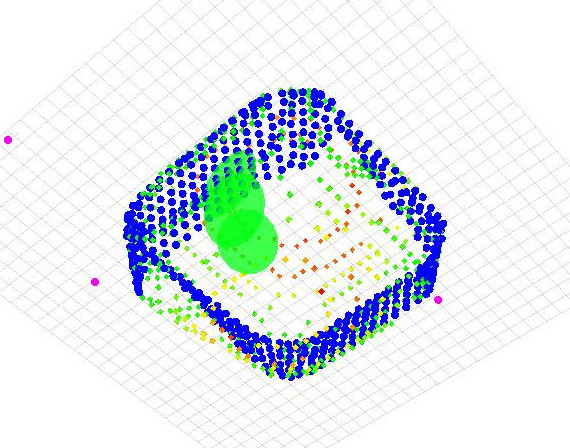
\includegraphics[width=0.45\textwidth]{next_best_touch.jpg}
  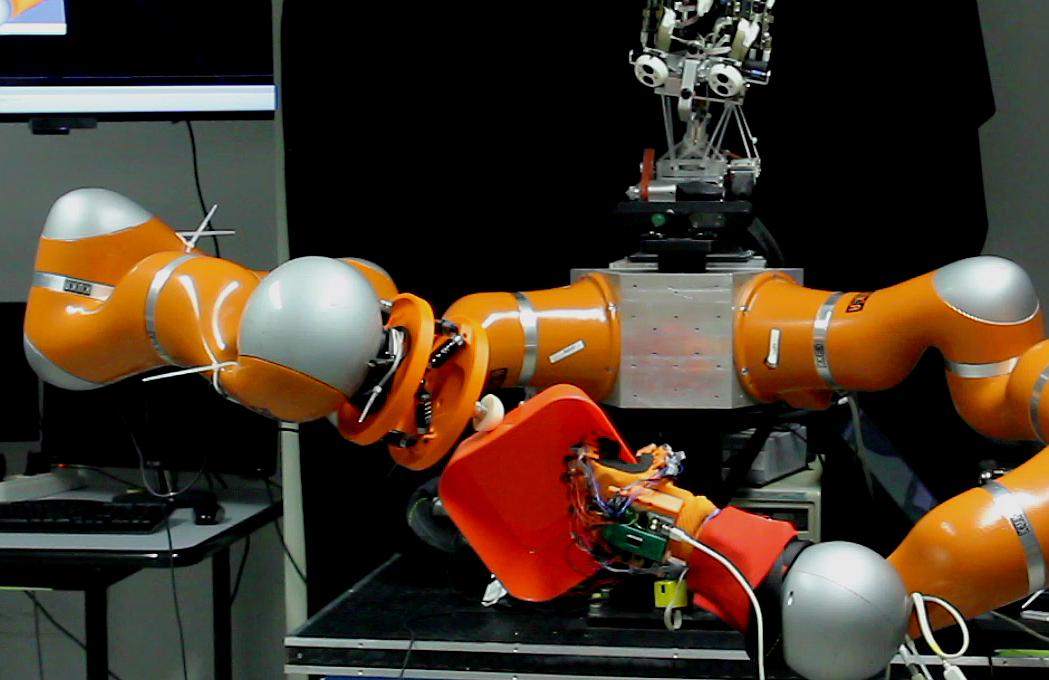
\includegraphics[width=0.53\textwidth]{intro_vito.png}
%}
\caption{The GPAtlasRRT strategy suggests touches (lighter green coloured disks) on the predicted surface. The predicted surface is shown as points colored from green to red according to higher or lower variance in the prediction, respectively, and the blue points are the initial partial view (left). Our Vito robot executing one of the recommended tactile actions (right). }
\label{fig:setup_solution}
\end{figure*}

% why the problem we are dealing with is important
Recovery of the surface properties of a new object is one of the most basic tasks in robot manipulation. This requires active exploration, using one or more modalities, to recover properties such as object shape, frictional coefficients, etcetera. Vision and active vision to support robotic grasping \cite{Kragic2002TechRep,nunez2013models,arruda16,kopicki2015ijrr,kootstra2012a} has been studied in depth. Humans also rely to a great extent on tactile information \cite{johansson92}, and there are a variety of works on how a robot should perform to tactile exploration during manipulation \cite{zito2013sequential,jentoft2014a,Bjorkman2013Enhancing,Hebert2013Next,Petrovskaya2011Global}. The goal of our work is to extend the set of methods employable for tactile exploration.

Active tactile perception needs were authoritatively spelled out by \cite{Bajcsy1988Active} in the 1980's and early perception algorithms date back to the same years \cite{Grimson1984JRR,Faugeras1983IJCAI,Shekhar1986ICRA,Bajcsy1989Machine}, but active touch lags behind active vision for two reasons. The first is technological: standardized touch sensors are not easily available and typically have to be hand crafted or modified for the specific robot and task. The second is intrinsic to touch itself, which requires the mechanical interaction of the sensor and the object being perceived. This inevitably leads to unexpected perturbations of the sensor and object and, which requires in turn complex control of the ongoing movement of the sensor: a requirement which is absent in vision.

Our scenario is motivated by tactile exploration when other sensor modalities, like vision, have already provided initial but incomplete information about object shape. From this initial, partial model we present a method to plan tactile exploration actions. This plan relies on the ability to make a hypothesis about where some point on the surface of the object is in space. This is tested, and then accepted or discarded after execution. Whether the evidence verifies or falsifies the hypothesis it improves the model of the object shape.

The object shape representation we employ is a probabilistic one and it is based on Gaussian Process (GP) \cite{Rasmussen2006Gaussian}, a machine learning formalism for nonlinear function regression that naturally provides a quantification of multi-modal uncertainty about object surface estimates, i.e. the variance of the estimate. This representation has previously been employed in surface modelling~\cite{Dragiev2011Gaussian,Bjorkman2013Enhancing, Sommer2014Bimanual}. The surface is implicitly defined, being the $0$-levelset of an \emph{unknown} function. It is handy to interpret it as a manifold and thus build our tactile exploration algorithm on top of recent results on sample-based exploration of general manifolds~\cite{Jaillet2013Path}. We can thus define hypotheses on where to sample next---next-best touch---to reduce uncertainty. In more detail, without the need to embed the manifold in its ambient space, we build a collection of charts (an atlas) that locally parameterizes it, and select among the points on the current atlas the one(s) fulfilling the search criteria: this represents the location where the next touch will be directed. Then, the growth of the atlas itself does not follow a predefined sequence of steps, but an RRT-like strategy is employed to devise directions to expand the atlas.
We propose a search criteria that looks for points on the estimated surface with a variance  larger than a pre-specified threshold. The expansion process is then repeated after the execution of the suggested touch. By repeated touches the robot should therefore converge on an estimated surface, such that any point on it has a variance smaller than this pre-specified threshold. This approach trades completeness in exploration for efficiency: the RRT drives the growth of the atlas toward regions of the object surface that are more uncertain, delaying the refinement of areas that have been already explored.

The terminating condition is met when no candidate for the next best touch is found by the GPAtlasRRT algorithm, which means the that object shape prediction meets the requirement on variability. Naturally, the smaller the threshold (i.e. the more accurate the model is required to be), the higher the number of touches required to converge. This threshold is the only input to the devised strategy, given either by a higher level module or the user.

The structure of the paper is as follows. In Sec.~\ref{sec:related} we first review previous work related to tactile exploration and object shape representation. In Sec.~\ref{sec:scope} we clearly state the problem we aim to solve and in Sec.~\ref{sec:solution} we present the envisioned approach for its solution. The experimental results and their discussion are presented in Sec.~\ref{sec:experiments}. Finally, conclusions and points deserving further attention are given in Sec.~\ref{sec:conclusions}.

% why tactile exploration is not so developed
% and what makes the problem harder that active vision

% why we propose touch (Bajcsy) and why ITS

% what is exactly our contribution

% RELATED WORK

% only localization

% also shape reconstruction
% they also use GP

% what are we doing more at least in surface exploration?
% we are exploiting the implicit manifold nature of GP representation
% and adapt efficient sample-based method for exploring the manifold in
% an intrinsic  way.



%General guidelines : \cite{Bajcsy1989Machine}
%
%Active visual perception: \cite{Bajcsy1988Active}
%
%Vision-based exploration is the most studied, perhaps due to its non-invasive nature, which avoids the contact between rigid bodies which is the cause of most headaches in physics modelling, simulation and control.
%
%As very well said by \cite{Petrovskaya2011Global}, even when initial works date back to the 80's, tactile perception has not been addressed as deeply as the non-invasive counterpart, visual perception. Besides the need of being actively controlled, tactile sensors typically required ad-hoc mechanical devices.
%
%``Touch-based perception has not been studied in as much depth
%as vision because standardized touch sensors are not as easily
%available. In many situations, tactile sensors have to be hand
%crafted specifically for the robot and the task. This complicates
%comparisons between methods and slows progress in tactile
%perception. However, recently there has been a surge of interest
%in the field due to the necessity of touch-based perception in
%service applications''
%
%Whereas \cite{Petrovskaya2011Global} is more interested in the object pose estimation problem, here we are more interested in the object shape modelling, sort of in the mapping of rather than localization in a SLAM problem.
%
%On active touch sensing \cite{Prescott2011Active}
%
%Differentiate from active touch for localization, here another example: \cite{Hebert2013Next}.
%
%Justify the use of a intrinsic tactile sensor over a tactile array.
%
%ITS are more precise and less noisy. It provides the contact normal directly in sensor frame.
%
%Tactile arrays provide multiple-point measurements. They do not provide directly the normal in sensor frame, forward kinematics is required over noisy joint measurements, or in fixed configurations that limit exploration mobility. Up to a point that a typically a complex framework is needed to exploit its grasping and touching properties % cite http://www.roboticsproceedings.org/rss09/p45.pdf?
%
%With ITS, the computation will be trivial. The disadvantage is that it is a single-point measurement. Poking strategies, like in~\cite{Petrovskaya2011Global}, or trajectories strategies like in~\cite{Rosales2014Active}.
%
%% They claim that touch sensing is low bandwith, local, sequential process with better signal-to-noise ratio than vision.
%
%% Vision is global, has high bandwidth, and is noisy. Touch is a low bandwidth, local, sequential process with better noise properties than vision.
%
%%% Finish the introduction with some motivation
%On how to do classification...
%
%Shape representation and descriptor review \cite{Zhang2004Review}
%
%In this work, we provide a systematic methodology to plan the next-best tactile exploratory action. The tactile exploratory action is intrinsically a contact hypothesis that need to be accepted or discarded after execution. Should the result be any of the two, it helps to improve the object shape prediction up to a pre-specified variability. In contrast to \cite{Bjorkman2013Enhancing}, we propose the same shape representation as descriptor for classification purposes using shape matching techniques~\cite{Belongie2002Shape}. The scope and problem statement is detailed in Sect.~\ref{sec:scope}. The proposed solution is broaden in Sect.~\ref{sec:solution}. The experimental results and discusion is presented in Sect.~\ref{sec:experiments}. Finally, the conclusions and points deserving further attention as given in Sect.~\ref{sec:conclusions}.
%%Reading the paper along watching the attached media is suggested for a better cath-up of the ideas. 